\documentclass{beamer}
\usepackage[utf8]{inputenc}
\usepackage[spanish, activeacute]{babel}
\usepackage{caption, subcaption}
\usepackage {amsmath, amssymb, bbm, stackrel, color, colortbl}
\usepackage{tikz}

\newcommand{\BigO}[1]{\ensuremath{\operatorname{O}\bigl(#1\bigr)}}

\usetheme{Boadilla}
%\useoutertheme{shadow}

% Para eliminar el footer
%\setbeamertemplate{footline}[page number]{}
% Los navigation symbols no sirven para nada
\setbeamertemplate{navigation symbols}{}

% Para poner la tabla de contenidos automaticamente al comienzo de cada seccion
%\AtBeginSection[]{\begin{frame}\frametitle{Tabla de contenidos}\tableofcontents[currentsection]\end{frame}}

% Customizacion de la tabla de contenidos
%\setbeamerfont{section number projected}{family=\rmfamily,series=\bfseries,size=\normalsize}
%\setbeamercolor{section number projected}{bg=black,fg=yellow}
%\setbeamertemplate{sections/subsections in toc}[ball]


% Title page
\title[RI]{Query Expansion with Random Embeddings}
\author[]{\\[4mm]Lucas Bernardi}
\date{January 2014}


\begin{document}

\frame{\titlepage}

\frame{\tableofcontents}

\section{Intro}

\begin{frame}
	\frametitle{Query Expansion}
	\framesubtitle{Problem Statement}
	\bigskip
	\begin{itemize}
	\item In the context of Information Retrieval, Query Expansion is a method to increase recall and/or precision by modifying a user query
  \item A specific case is the expansion of each term to related terms, increasing recall (and precision as a side effect)
  \item Example: User query: soccer, expanded query: soccer football maradona
  \item  The Problem: Learn to expand terms
	\end{itemize}
\end{frame}

\begin{frame}
	\frametitle{A General Approach}
	\begin{block}{The distributional hypothesis}
    Words with similar distributional properties have similar meanings.
  \end{block}
\bigskip
	\begin{block}{The geometric metaphor of meaning}
  Meanings are locations in a semantic space, and semantic similarity is proximity between the locations.
  \end{block}
\end{frame}


\begin{frame}
	\frametitle{The Vector Space Model Approach}
	\framesubtitle{A solution}
  \begin{itemize}
    \item	An algebraic model for information retrieval and NLP
    \item	Defines a vector space to represent terms
    \item	Defines a dimension for each unique term
    \item	Each term is represented by a semantic vector
    \item Each component of a semantic vector is the weight of the represented term in the direction of the dimension term
    \item Weights are a design decision, TF-IDF is widely used
    \item Compute the related terms of a given term as its k-nearest neighbors
    \item The vector distance/similarity measure is a design decision, cosine similarity is widely adopted
  \end{itemize}
\end{frame}

\begin{frame}
	\frametitle{The Vector Space Model Approach}
	\framesubtitle{Some drawbacks}
  \begin{itemize}
    \item	Curse of dimensionality
    \item	Sparse vectors
    \item	Dynamic vector space
      \end{itemize}
      \bigskip
      Alternatives
  \begin{itemize}
    \item	Use documents as dimensions: Less dimensions, but still sparse vectors and still a dynamic space
    \item	Use topics as dimensions: Less dimensions, dense vectors and fixed space, but how can we define topics and assign weights?  Latent Semantic Analysis
  \end{itemize}
\end{frame}

\section{Random Projections}

\subsection{The Random Projections Approach}
\begin{frame}
	\frametitle{The Random Projections Approach}
	\framesubtitle{Overcoming drawbacks}
	\begin{itemize}
	\item Use a random low dimensional space
	\item Less dimensions, dense vectors, fixed space
	\item No semantic assigned to dimensions
	\item But, how are weights assigned?
	\end{itemize}
\end{frame}

\begin{frame}
	\frametitle{The Random Projections Approach}
	\framesubtitle{A simple algorithm }
	\begin{itemize}
		\item Assign a random k-dimensional vector to each term (index vector)
		\item Allocate a null k-dimensional vector to each term (semantic vector)
		\item For each sentence in the corpus compute bigrams $(left$ $right)$
		\item For each bigram 
		\begin{itemize}
		  \item $semantic(left)$ += $index(right)$
		  \item $semantic(right)$ += $index(left)$
		\end{itemize}
	\end{itemize}
\end{frame}	

\begin{frame}
	\frametitle{The Random Projections Approach}
	\framesubtitle{A simple algorithm: Illustration}
\end{frame}	

\begin{frame}
	\frametitle{The Random Projections Approach}
	\framesubtitle{A simple algorithm: a formal description}

Given a text documents corpus $D$ we define \\
$\mathbb{T}=\{\text{All terms in } D\}$, $t =  \left\vert{\mathbb{T}}\right\vert$ \\
$\mathbb{C} = \{\text{All contexts in } D\}$, where a context is a set of terms \\
$t$ random $k$-dimensional vectors $r_i, 1\leq i\leq t$,  $\mathbb{R} = \{r_i\}$ \\
$t$ semantic $k$-dimensional vectors $s_i, 1\leq i\leq t$,  $\mathbb{S} = \{s_i\}$ \\
A mapping $S:w \in \mathbb{T} \rightarrow  \mathbb{S}$, which maps a term to its semantic vector \\
A mapping $R:w \in \mathbb{T} \rightarrow  \mathbb{R}$, which maps a term to its random vector \\
A mapping $C:w \in \mathbb{T} \rightarrow  \{\mathbb{C}\}$, which maps a term to a set containing all the contexts it appears \\
Then we can express the semantic vector assigned to the term $w$ as: \\
\begin{equation}
s_w =\sum\limits_{c \in C(w)} \sum\limits_{p \in c} R(p)
\end{equation}
\end{frame}

\subsection{Algebraic Interpretation}

\begin{frame}
  	\frametitle{The Random Projections Approach}
  	\framesubtitle{Algebraic Interpretation}
  	
Defining a co-occurrence matrix $M \in \mathbb{Z}^{t \times t} $, $M_{ij} = \sum\limits_{c \in C(t_i)} \mathbbm{1}_c (t_j)$ \\
Each cell $i, j$ in $M$ counts the amount of contexts in $D$ containing the $i$th and $j$th terms\\
Introducing a random matrix $R \in \mathbb{Z}^{t \times k} $,  $R_i = R(t_i)$, that is, all random vectors as rows, we can express a semantic vector as:\\
\begin{equation}
s_i =\sum\limits_{j=1}^{t} R(t_j)M_{ij} =\sum\limits_{j=1}^{t} R_jM_{ij}
\end{equation}
If we also define the semantic matrix $S \in \mathbb{Z}^{t \times k} $ with $S_i = s_i$, that is, all semantic vectors as rows, we can finally write:\\
\begin{equation}
S=MR
\end{equation}
\end{frame}


\begin{frame}
  	\frametitle{The Random Projections Approach}
  	\framesubtitle{Algebraic Interpretation}
  	\begin{equation}
S=MR
\end{equation}
\begin{itemize}
  \item This equation is a mathematical expression of our initial algorithm
  \item Semantic vectors are just the matrix product of the VSM vectors and a random matrix
  \item The algorithm is simply reducing the dimensionality of the VSM vectors
  \item For certain distributions of R, R is a nearly orthogonal
  \item Then we can interpret this product as the projection of the VSM vectors onto a random lower dimensional space
\end{itemize}
\end{frame}


\subsection{Theoretical support}
\begin{frame}
  	\frametitle{The Random Projections Approach}
  	\framesubtitle{Theoretical support}
  	\begin{block}{The Johnson and Lindenstrauss Lemma}
Given $\epsilon > 0$ and an integer $n$, let $k$ be a positive integer such that $k \geq k_{0} = \BigO{\epsilon^{-2}  \log n} $. For every set $\mathbb{P}$ of $n$ points in $\mathbb{R}^{d}$ there exists $f: \mathbb{R}^{d}  \rightarrow \mathbb{R}^{k}$ such that for all $u,v \in \mathbb{P}$\\
  	\bigskip
  	\centering
  	$(1-\epsilon)\lVert u-v \rVert^{2} \le \lVert f(u)-f(v) \rVert^{2}\le (1+\epsilon)\lVert u-v \rVert^{2}$\\
  	\end{block}
\end{frame}
\begin{frame}
  	\frametitle{The Random Projections Approach}
  	\framesubtitle{Theoretical support}
\begin{block}{Achlioptas Theorem}

  	  Let $\mathbb{P}$ be an arbitrary set of $n$ points in $R^{d}$ represented as an $n \times d$ matrix $A$. Given $\epsilon, \beta >0$ let $k_{0}=\frac{4+2\beta}{\frac{\epsilon^{2}}{2}-\frac{\epsilon^{3}}{3}}\log n$. For integer $k \ge_{0}$, let $\mathbb{R}$ be a $d \times k$ random matrix with $R(i,j)=r_{ij}$, where $\{r_{ij}\}$ are independent random variables from either one of the following two probability distributions:\\

\begin{minipage}[b]{0.45\linewidth}
\[
 r_{i,j} =
  \begin{cases}
   +1 & \text{with probability } \frac{1}{2} \\
  -1 & \text{with probability } \frac{1}{2} \\
  \end{cases}
\]  	  
\end{minipage}
\begin{minipage}[b]{0.45\linewidth}
\[
 r_{i,j} = \sqrt{3}\times 
  \begin{cases}
   +1 & \text{with probability } \frac{1}{6} \\
   0 & \text{with probability } \frac{2}{3} \\
  -1 & \text{with probability } \frac{1}{6} \\
  \end{cases}
\]
\end{minipage}\\
\bigskip
Let $E=\frac{1}{\sqrt{k}}AR$. Let $f: \mathbb{R}^{d}\rightarrow \mathbb{R}^{k}$ map the $i^{th}$ row of $A$ to the $i^{th}$ row of $E$.
\bigskip
With probability at least $1-n^{-\beta}, for all u, v \in \mathbb{P} $

\centering
$(1-\epsilon)\lVert u-v \rVert^{2} \le \lVert f(u)-f(v) \rVert^{2}\le (1+\epsilon)\lVert u-v \rVert^{2}$\\
\end{block}
\end{frame}

\section{Empirical Study}
\subsection{Relative Error}

\begin{frame}
\frametitle{Empirical Study}
\framesubtitle{Relative error}

\centering
$(1-\epsilon)\lVert u-v \rVert^{2} \le \lVert f(u)-f(v) \rVert^{2}\le (1+\epsilon)\lVert u-v \rVert^{2}$\\
\medskip
$1-\epsilon \le \frac{\lVert f(u)-f(v) \rVert^{2}}{\lVert u-v \rVert^{2} }\le 1+\epsilon$\\
\medskip
$-\epsilon \le \frac{\lVert f(u)-f(v) \rVert^{2}}{\lVert u-v \rVert^{2}} - 1\le \epsilon$\\
\medskip
$-\epsilon \le \frac{\lVert f(u)-f(v) \rVert^{2}-\lVert u-v \rVert^{2}}{\lVert u-v \rVert^{2}}\le \epsilon$\\
  	
\end{frame}



\begin{frame}
\frametitle{Empirical Study}
\framesubtitle{Set up}
\begin{itemize}
  \item Natural language corpus with 140000 unique terms
  \item Filtered out low frequency terms
  \item Plain VSM vectors (original space is represented by the co-occurrence matrix)
  \item Random space dimension from 100 to 2000
  \item Random space generated with the sparse Achlioptas distribution
  \item Measured relative error ($\epsilon$) between high-dimensional vectors and low dimensional vectors
\end{itemize}
\end{frame}


\begin{frame}
\frametitle{Empirical Study}
\framesubtitle{Results}
  		\begin{figure}
		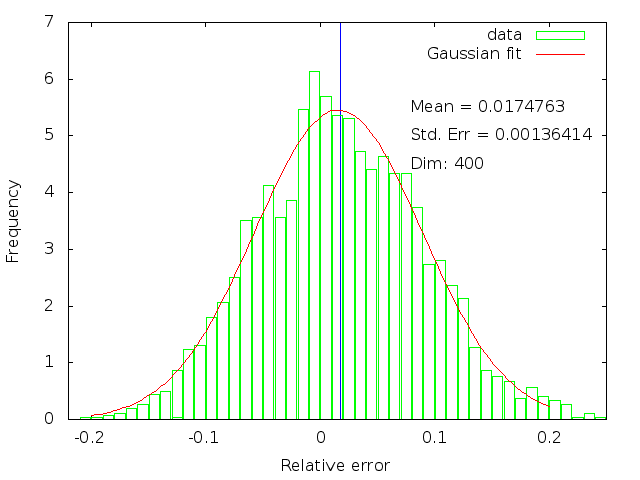
\includegraphics[scale=0.46]{histogram400.png}
	\end{figure}
\end{frame}

\begin{frame}
\frametitle{Empirical Study}
\framesubtitle{Results}
  		\begin{figure}
		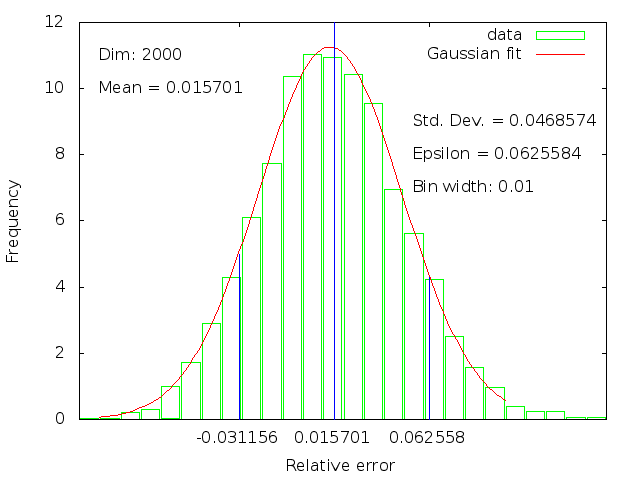
\includegraphics[scale=0.46]{histogram2000.png}
	\end{figure}
\end{frame}

\begin{frame}
\frametitle{Empirical Study}
\framesubtitle{Results}
  		\begin{figure}
		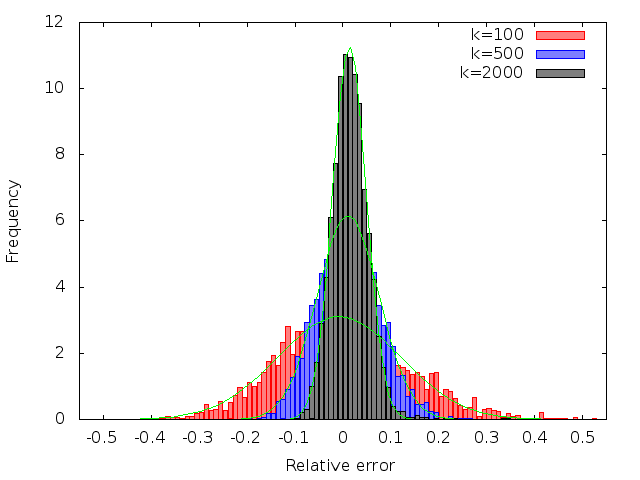
\includegraphics[scale=0.46]{histogramAll.png}
	\end{figure}
\end{frame} 

\begin{frame}
\frametitle{Empirical Study}
\framesubtitle{Results}
 		\begin{figure}
		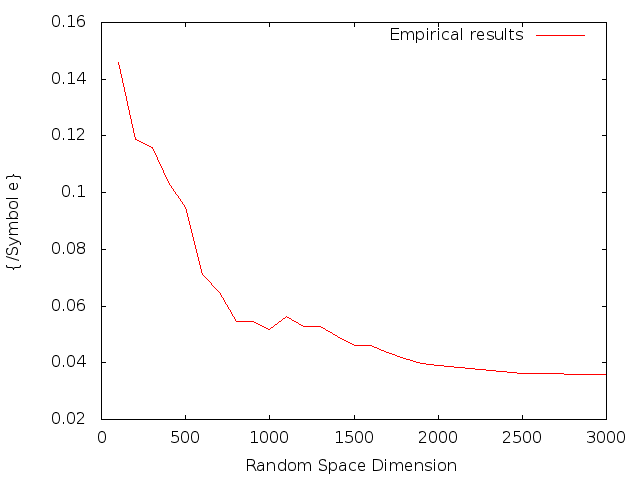
\includegraphics[scale=0.46]{epsilon.png}
	\end{figure}
\end{frame} 
\begin{frame}
\frametitle{Empirical Study}
\footnotesize
\begin{tikzpicture}
    \draw (0, 0) node[inner sep=0] {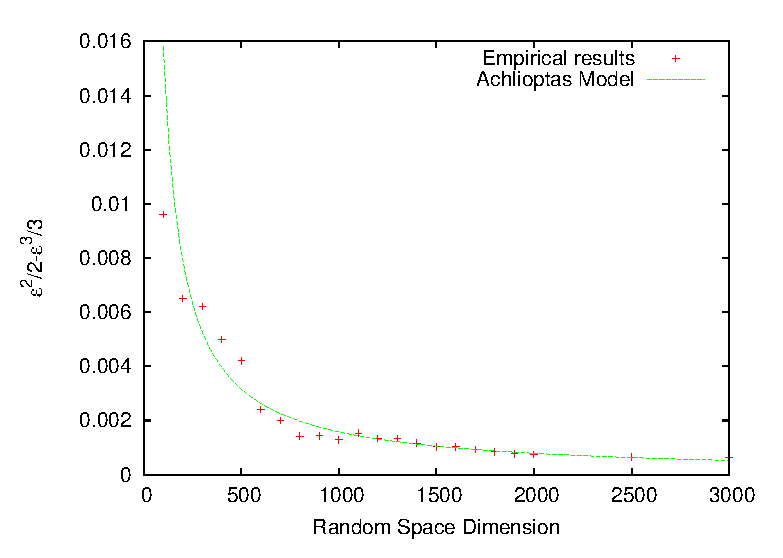
\includegraphics[scale=0.9]{epsilonFit.eps}};
    \draw (1, 1) node {Achlioptas Model:  $p(\epsilon)=\frac{4+2\beta}{k_{0}}\log n$};
    \draw (1, 2) node {$p(\epsilon) = \frac{\epsilon^{2}}{2}-\frac{\epsilon^{3}}{3}$};
\end{tikzpicture}
\end{frame} 

\begin{frame}
	\frametitle{Resultados}
	\framesubtitle{Comparación}	
\begin{itemize}
\item Matrices de confusión \\
\smallskip
\small
\begin{tabular}{ l | l |  l }                     
   & Actual Match & Actual Unmatch \\ \hline
Det says Matched & $6212$ (tp) & $0$ (fp)\\ \hline
Det says Unmatched & $40862$ (fn) & $4775173$ (tn)\\
  \hline  
Prob says Matched & 39628 (tp) & $197$ (fp)\\ \hline
Prob says Unmatched & 7446 (fn) & $4774976$ (tn)\\
  \hline  
\end{tabular}
\smallskip
\item Metricas \\
\smallskip
\begin{tabular}{ l | l | l |  l }                     
   & Precision & Recall & F-Score\\ \hline
Det & $1$  & $0.22$ & $0.36$ \\ \hline
Prob & $0.99$ & $0.84$ & $0.91$ \\   \hline  
\end{tabular}
\end{itemize}
\end{frame}


\begin{frame}
	\frametitle{Resultados}
	\framesubtitle{Conclusión}	
	\begin{block}{Conclusión}
		\begin{itemize}
		\item A costa de menos del $1\%$ de precision, Prob, detecta 4 veces mas Matches correctos que Det.
		\item Prob puede ser mejorado en varios aspectos incrementando tanto la precision, como la capacidad de detectar matches correctos, mientras que no es claro de que forma se puede mejorar el recall de Det.
		\end{itemize}
  \end{block}
\end{frame}



\section{Análisis}

\begin{frame}
	\frametitle{Similitud}
	\framesubtitle{Un enfoque intuitivo}
		\begin{block}{Idea general}
	Fichas similares, representan al mismo hotel, fichas disímiles representan hoteles diferentes.
	  \end{block}
	\begin{itemize}
	  \item Definiciones:
	  \begin{itemize}
	    \item 
			$\mathbb{F}: \text{conjunto de todas las fichas de hoteles}$ \\
			\item
      $\mathbb{D}: \{Match, Unmatch, Review\}$ (conjunto de decisiones posibles)\\
      \item
      $L:(a \in \mathbb{F}, b \in \mathbb{F}) \rightarrow  \mathbb{D}$ (función decisión)
    \end{itemize} 
		\item Se construye una función de similitud entre fichas de hoteles: 
      $S:(a \in \mathbb{F}, b \in \mathbb{F}) \rightarrow  \mathbb{R}$ \\
		\item $S$ es una función escalar, cuando mayor es el valor de la función, mas similares son sus argumentos.
		\item Se determinan umbrales $m, u \in \mathbb{R}, m\geq u$ de similitud:
	\small	
$$
L(a,b) =
\begin{cases}
Match & \text{si }S(a,b)>m \\
Review & \text{si }u\leq S(a,b)\leq m \\
Unmatch & \text{si }S(a,b)<u
\end{cases}
$$
\end{itemize}
\end{frame}

\begin{frame}
	\frametitle{Similitud}
	\framesubtitle{Limitaciones}
	\begin{itemize}
		\item La similitud entre fichas no necesariamente es un buen indicador de matching: dos fichas pueden ser muy similares y representar hoteles diferentes.
		\item Imperfecciones en la función de similitud: para dos fichas $a$ y $b$ muy similares $S(a, b)$ es pequeño.
		\item La función de similitud es naturalmente vectorial. Convertirla en escalar inevitablemente introduce ruido.
\end{itemize}
\end{frame}
  
\begin{frame}
	\frametitle{Fellegi y Sunter}
	\framesubtitle{Un modelo probabilístico}
	\small
	\begin{block}{Idea general}
      Se estudia la distribución de la similitud en Matches y Unmatches. 
	\begin{itemize}
      \item Valores de similitud con frecuencia alta en Matches, pero baja en Unmatches: Match.
      \item Valores de similitud con frecuencia alta en Unmatches, pero baja en Matches: Unmatch.
      \item Valores de similitud con la misma frecuencia en  Matches y Unmatches: Review.
    \end{itemize} 
	\end{block}
  Definiciones:
	  \begin{itemize}
      \item
      $\mathbb{P}: \mathbb{F}\times \mathbb{F}$ producto cartesiando de $\mathbb{F}$
      \item
      $\mathbb{M}: \{(a,b) \in P  \mid a\text{ representa el mismo hotel que }b\}$
      \item
      $\mathbb{U}: \{(a,b) \in P  \mid a\text{ no representa el mismo hotel que }b\}$
      \item
      $\mathbb{P} = \mathbb{U} \cup \mathbb{M}, \mathbb{U} \cap \mathbb{M} = \emptyset$
    \end{itemize} 
\end{frame}

\begin{frame}
	\frametitle{Fellegi y Sunter}
	\framesubtitle{Un modelo probabilístico: Similitud}
	  \begin{itemize}
      \item La función similitud es vectorial:
      $\gamma:(a \in \mathbb{F}, b \in \mathbb{F}) \rightarrow  \mathbb{X}^{n}$ \\
      \item Cada componente de la función $\gamma$ es una función de comparación sobre un campo de la ficha (nombre del hotel, dirección, etc.) 
      \item Estas componentes no son necesariamente escalares:
      $\gamma(a, b) = <\gamma_1(a, b), \gamma_2(a, b), ..., \gamma_n(a, b)>$
      \item Para cada valor posible de la función $\gamma$, se definen los siguientes parámetros:
      $m(\gamma) = P(\gamma(a, b)=\gamma | \text{ a representa el mismo hotel que b })$
      $u(\gamma) = P(\gamma(a, b)=\gamma | \text{ a no representa el mismo hotel que b })$
      \item $m(\gamma_0)$ nos dice que tanto podemos sospechar de un Match al observar $\gamma_0$
      \item $u(\gamma_0)$ nos dice que tanto podemos sospechar de un Unmatch al observar $\gamma_0$    
      \end{itemize} 
\end{frame}

\begin{frame}
	\frametitle{Fellegi y Sunter}
	\framesubtitle{Un modelo probabilístico: Regla de decisión}
	  \begin{itemize}
      \item Los parámetros $m$ y $u$ se combinan en un único peso:
      $w(\gamma_0) = m(\gamma_0)/u(\gamma_0)$
      \item A mayor $w$ mayor certeza de estar frente a un Match.
      \item Se determinan umbrales de peso $w_m$, $w_u$, para tomar las decisiones:
      $$
L(a,b) =
\begin{cases}
Match & \text{si }w(\gamma(a,b))>w_m \\
Review & \text{si }w_u\leq w(\gamma(a,b))\leq w_m \\
Unmatch & \text{si }w(\gamma(a,b))<w_u
\end{cases}
$$
\item Esta regla de decisión minimiza la región de revisión humana.
\item La estimación de parámetros $m$ y $u$ se realizó mediante Maximum Likelihood Estimation.
\item Los umbrales fueron determinados por cross validation.
    \end{itemize} 
\end{frame}

\begin{frame}
	\frametitle{Fellegi y Sunter}
	\framesubtitle{Mejoras}
	  \begin{itemize}
      \item La regla de decisión es muy robusta a imperfecciones en la función de similitud
      \item A mejor función de similitud mejor rendimiento 
      \item Los pesos $w=m/u$ pueden calcularse de otra manera (minimizar el error)
      \item Los parámetros $u$ y $m$ pueden estimarse son métodos no supervisados
      \item La regla de decisión puede ser muy diferente (clasificación lineal general)
          \end{itemize} 
\end{frame}

\begin{frame}
	\frametitle{Fellegi y Sunter}
	\framesubtitle{Ilustración}
	\begin{center}
\end{center}
\end{frame}

\begin{frame}
	\frametitle{Evaluation set}
	Datos históricos: pares matcheados, pares unmatcheados
	
	  \begin{itemize}
\item Problemas
  \begin{itemize}
    \item Volumen insuficiente 
	  \item Sesgados: solo pares con determinadas (pero desconocidas) características de similitud
	  \item Mucho ruido (falsos matches, falsos unmatches)
	  \item Proporción de matches y unmatches no realista
	\end{itemize}  
\item Soluciones	


  \begin{itemize}
	  \item Reduccion de ruido: ejecuciones iniciales del modelo probabilístico determinaron candidatos a revisión humana que fueron corregidos
	  \item Incremento de volumen, reducción de sesgo: clausura bajo transitividad de matches
	  \item Incremento de volumen, reducción de sesgo, corrección de proporción entre clases: complemento a producto cartesiano.
	  \item El complemento a producto cartesiano produce ruido sistemático por generar falsos unmathces
	  \item Reduccion de ruido sistemático: Fellegi Sunter sobre clases de equivalencia.
	 \end{itemize}

\end{itemize}

	
\end{frame}


\begin{frame}%[allowframebreaks]
  \frametitle{Referencias}    
  \begin{thebibliography}{10}
  \beamertemplatearticlebibitems
  \bibitem{Fellegi&Sunter1969}
    Ivan P. Fellegi y Alan B. Sunter
    \newblock {\em A Theory for Record Linkage}.
    \newblock {\small Journal of the American Statistical Association Volume 64, Issue 328, 1969.}
  \beamertemplatearticlebibitems
  \bibitem{Deerwester1990}
    S.~Deerwester, et al.
    \newblock {\em Indexing by latent semantic analysis.}
    \newblock {\small JASIS 41.6 (1990): 391-407.}
  \beamertemplatearticlebibitems
  \bibitem{Kanerva2000}
    P.~Kanerva, et al.
    \newblock {\em Random indexing of text samples for latent semantic analysis.}
    \newblock {\small Proceedings of the 22nd annual conference of the cognitive science society. Vol. 1036. 2000.}
  \beamertemplatearticlebibitems
  \bibitem{Achlioptas2003}
    D.~Achlioptas.
    \newblock {\em Database-friendly random projections: Johnson-Lindenstrauss with binary coins.}
    \newblock {\small Journal of computer and System Sciences 66.4 (2003): 671-687.}
  \end{thebibliography}
\end{frame}

\end{document}
